\section{LOGICAL MODEL STRUCTURE}\label{sec:dataware}

The logical model of the data warehouse is a snowflake schema. It consists of a total amount of 8 different tables, 3 of those being fact tables. Trivial dimensions like Date and Time will not be described in depth.

\begin{figure*}[tb]
\centering
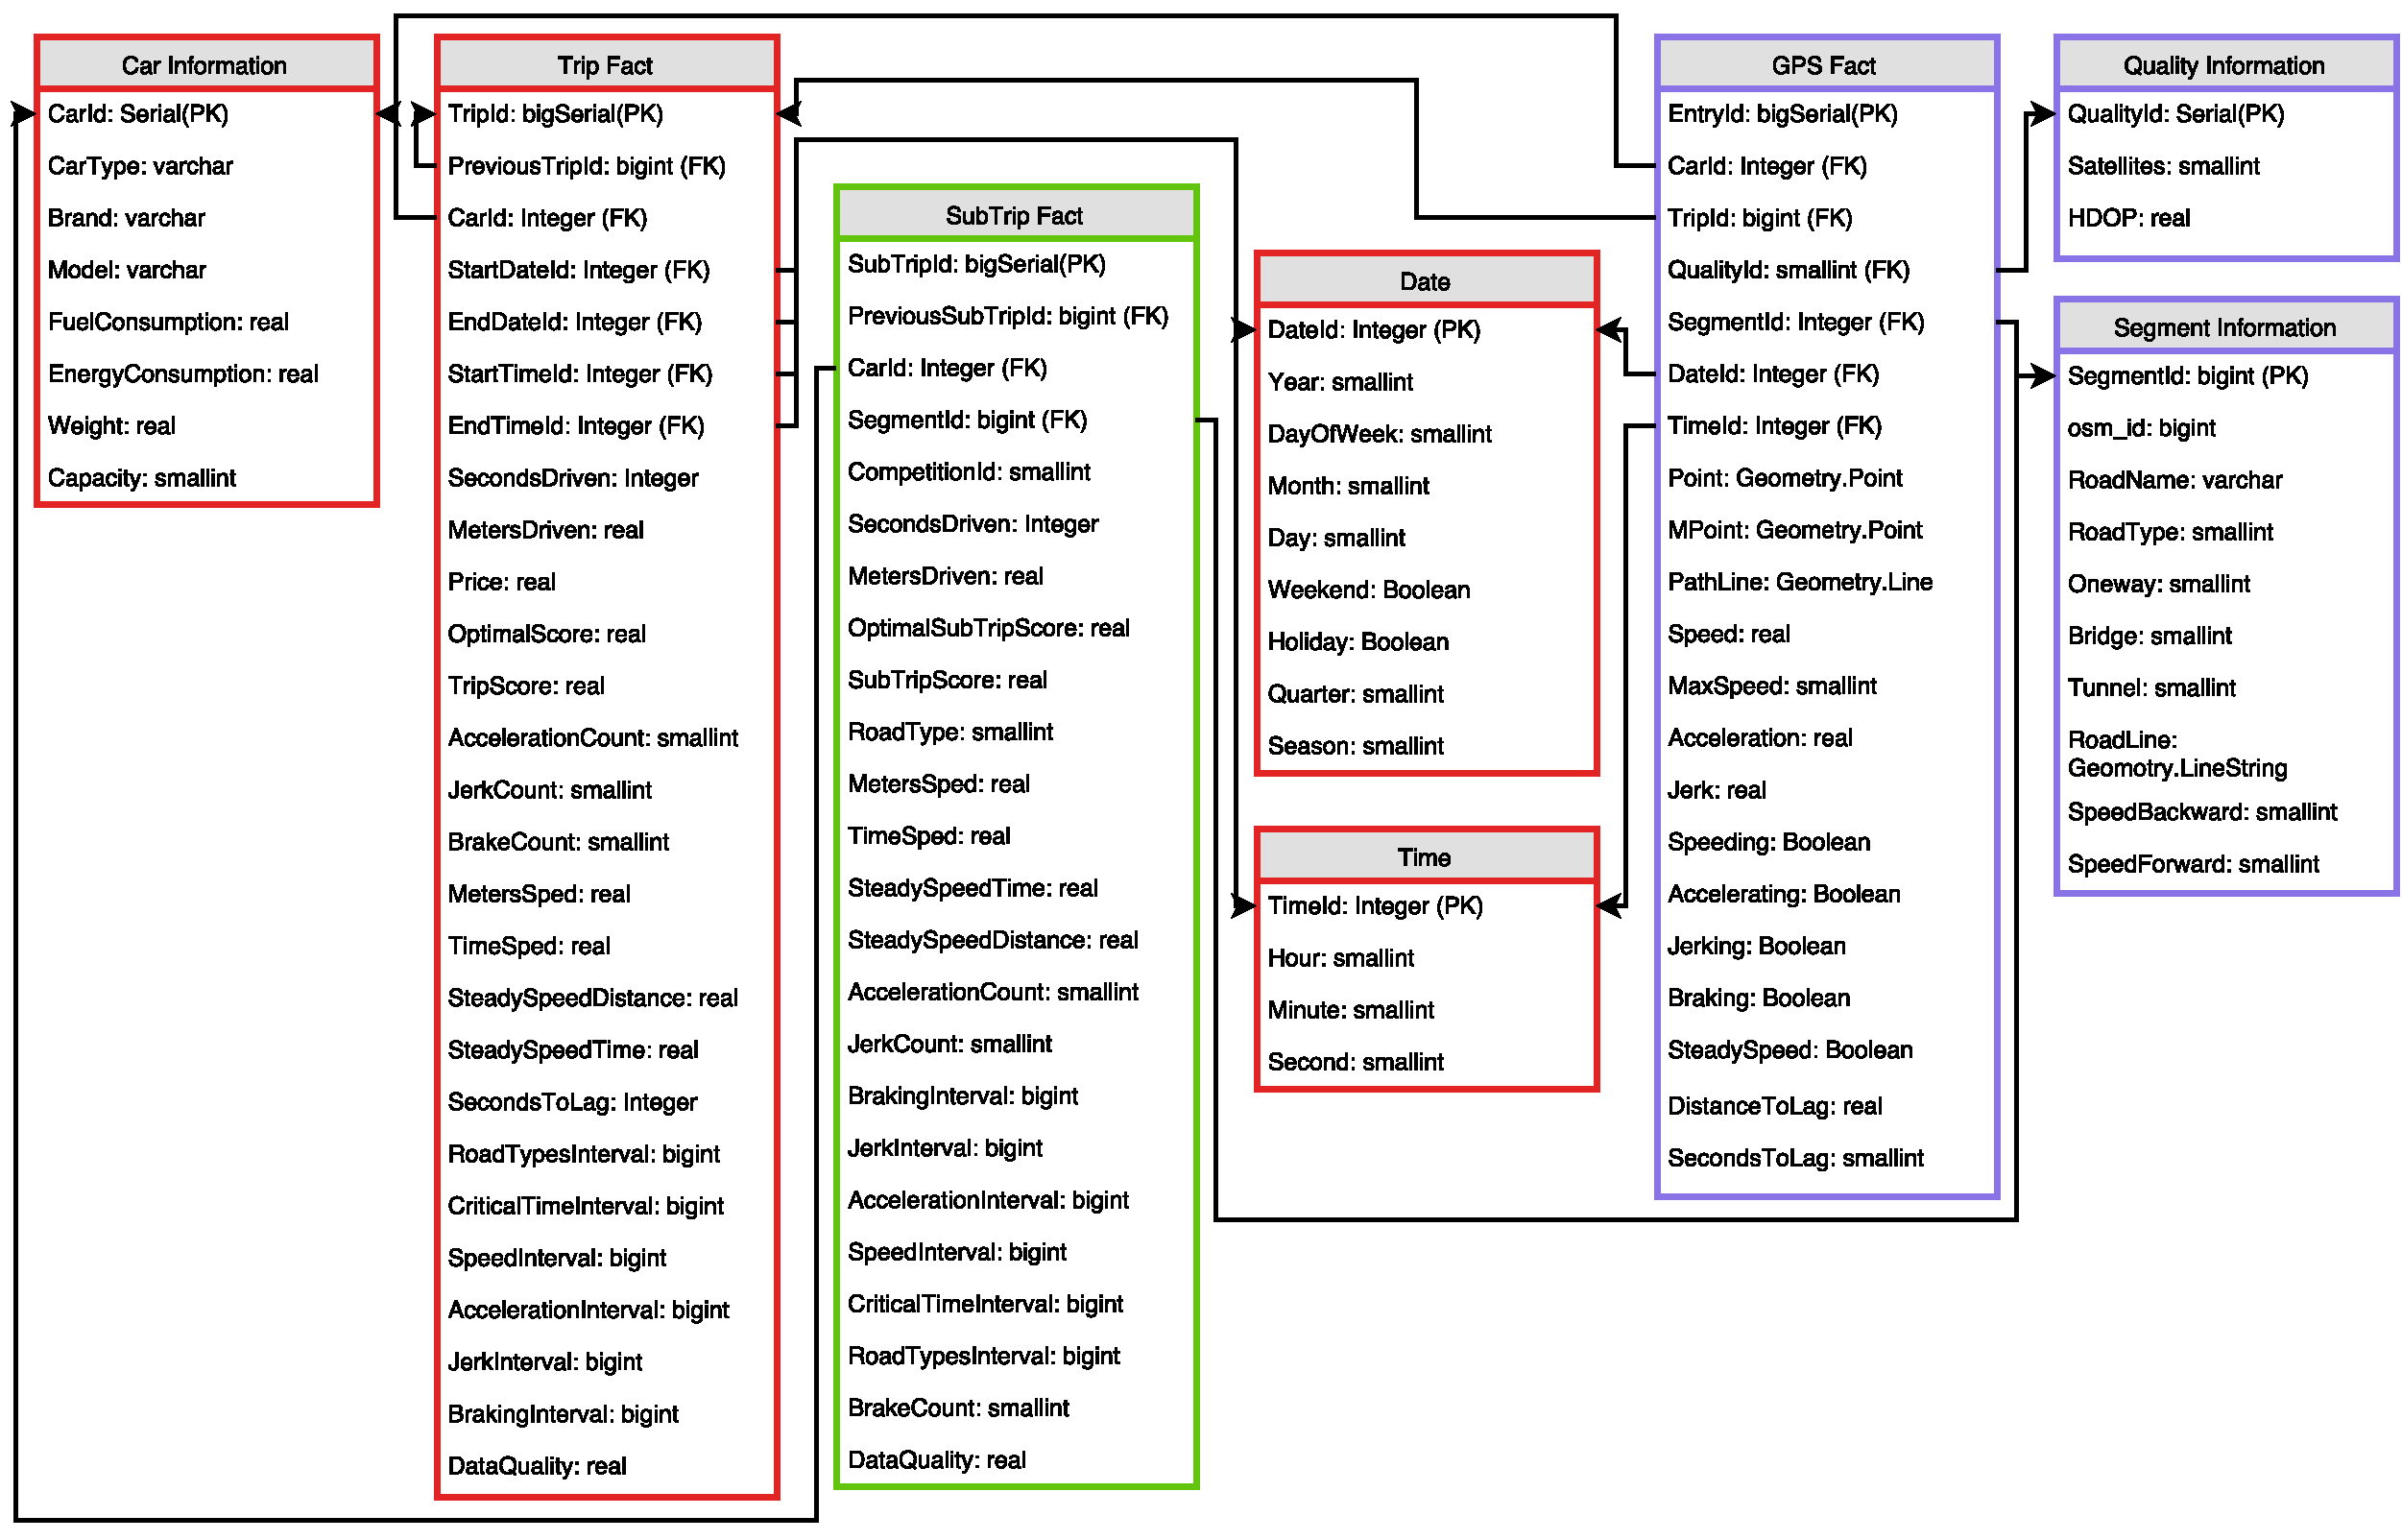
\includegraphics[width=0.9\textwidth]{Pictures/ERDiagram}
\caption{Logical Model of the Data Warehouse}
\label{fig:datawarehouse}
\end{figure*}

\subsection{Fact Hierarchy}

First, confirm that you have the correct template for your paper size. This template has been tailored for output on the US-letter paper size. Please do not use it for A4 paper since the margin requirements for A4 papers may be different from Letter paper size.

\subsection{Information Tables}

\textbf{Car Information} is a support table holding valid information about the users car. The data is valuable to the insurance company, if not for actual insurance calculations, then for statistical use. The data is of a relation 1 to many tripfacts, subtripfacts or gpsfacts, meaning each of these must have a link to an entry in Car Information. This is important due to the insurance policy is per car rather than per person.

\textbf{Quality Information} is a support table which determines the quality of the given gpsfact. The table contains information on the Horizontal-Dilution-of-Position(HDOP) and the amount of satellites covering the car. Whenever we encounter a new unseen combination of the two, we create an entry in the database. Entries are mapped 1 to many gpsfacts because of this, but we reduce the amount of duplicated information.

\textbf{Segment Information} is the last support table and it has the entire road network of Denmark from openstreetmap. We have kept the osm_id to make it possible for cooperation and better integration in the future. Segment Information is related 1 to many to both subtripfacts and gpsfacts.

\subsection{Color Divisions}